\documentclass{article}
\usepackage[T1]{fontenc}
\usepackage{helvet}
\renewcommand{\familydefault}{\sfdefault}
\usepackage{amsmath,amssymb}
\usepackage{sansmath}
\usepackage{tikz}
\usetikzlibrary{arrows.meta,fit,calc,positioning}
\pagestyle{empty}
\definecolor{acc}{HTML}{1F4E79}
\newsavebox{\figbox}
\begin{document}
\sansmath\fontsize{7}{8.4}\selectfont
\sbox{\figbox}{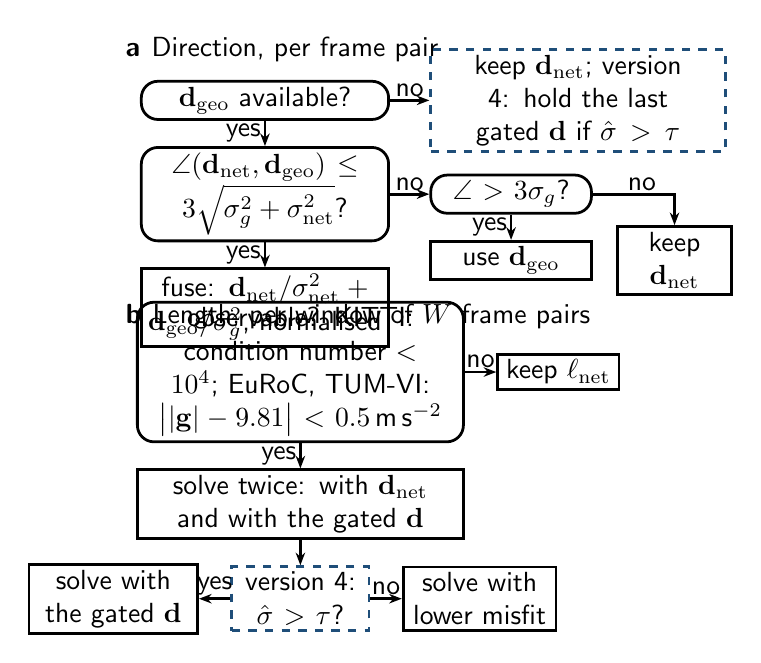
\begin{tikzpicture}[>={Stealth[length=1.6mm]}, every path/.style={line width=1pt}, node distance=3.2mm,
  q/.style={draw, rounded corners=6pt, align=center, inner sep=2pt, text width=#1},
  q/.default=30mm,
  a/.style={draw, align=center, inner sep=2pt, text width=#1},
  a/.default=19mm,
  v4/.style={draw=acc, dashed, align=center, inner sep=2pt, text width=#1},
  v4/.default=19mm,
  yn/.style={inner sep=1pt}]
\node[anchor=west] (ta) at (-1.9,0.35) {\textbf{a}\hspace{4pt}Direction, per frame pair};
\node[q] (d1) at (0,-0.3) {$\mathbf d_\mathrm{geo}$ available?};
\node[q, below=of d1] (d2) {$\angle(\mathbf d_\mathrm{net},\mathbf d_\mathrm{geo})\le 3\sqrt{\sigma_g^2+\sigma_\mathrm{net}^2}$?};
\node[a, below=of d2, text width=30mm] (fuse) {fuse: $\mathbf d_\mathrm{net}/\sigma_\mathrm{net}^2+\mathbf d_\mathrm{geo}/\sigma_g^2$, normalised};
\node[q, right=5mm of d2, text width=19mm] (d3) {$\angle > 3\sigma_g$?};
\node[a, below=of d3] (geo) {use $\mathbf d_\mathrm{geo}$};
\node[a, right=3mm of geo, text width=13mm] (net1) {keep $\mathbf d_\mathrm{net}$};
\node[v4, right=5mm of d1, text width=36mm] (nogeo) {keep $\mathbf d_\mathrm{net}$; version 4: hold the last gated $\mathbf{d}$ if $\hat\sigma>\tau$};
\draw[->] (d1) -- node[yn, above]{no} (nogeo);
\draw[->] (d1) -- node[yn, left]{yes} (d2);
\draw[->] (d2) -- node[yn, left]{yes} (fuse);
\draw[->] (d2) -- node[yn, above]{no} (d3);
\draw[->] (d3) -- node[yn, left]{yes} (geo);
\draw[->] (d3.east) -| node[yn, pos=0.3, above]{no} (net1.north);
\node[anchor=west] (tb) at (-1.9,-3.05) {\textbf{b}\hspace{4pt}Length, per window of $W$ frame pairs};
\node[q, text width=40mm] (l1) at (0.45,-3.75) {observable? KITTI: condition number $<10^4$; EuRoC, TUM-VI: $\big||\mathbf{g}|-9.81\big|<0.5$\,m\,s$^{-2}$};
\node[a, right=4mm of l1, text width=14mm] (lnet) {keep $\ell_\mathrm{net}$};
\node[a, below=of l1, text width=40mm] (solve) {solve twice: with $\mathbf d_\mathrm{net}$ and with the gated $\mathbf{d}$};
\node[v4, below=of solve, text width=16mm] (t2) {version 4: $\hat\sigma>\tau$?};
\node[a, left=4mm of t2, text width=20mm] (gsol) {solve with the gated $\mathbf{d}$};
\node[a, right=4mm of t2, text width=18mm] (mis) {solve with lower misfit};
\draw[->] (l1) -- node[yn, above]{no} (lnet);
\draw[->] (l1) -- node[yn, left]{yes} (solve);
\draw[->] (solve) -- (t2);
\draw[->] (t2) -- node[yn, above]{yes} (gsol);
\draw[->] (t2) -- node[yn, above]{no} (mis);
\end{tikzpicture}}
\hoffset=-1in \voffset=-1in
\pdfpagewidth=\wd\figbox
\pdfpageheight=\ht\figbox \advance\pdfpageheight by \dp\figbox
\shipout\copy\figbox
\end{document}
